\documentclass[11pt,letterpaper]{article}


% Packages
\usepackage{authblk} % author affiliations
\usepackage{graphicx} % graphics
\usepackage{amsmath, amssymb} % mathematical symbols
\usepackage{natbib} % bibliography
\usepackage[margin=1in]{geometry} % margins
\usepackage{lineno} % line numbers
\usepackage{setspace} % linespacing
\usepackage{hyperref} % For hyperlinks

% Set 1.5 spacing
\setstretch{1.5}


% Set citation style
\setcitestyle{numbers} 

% Metadata
\title{Time-series modeling of epidemics in complex populations: detecting changes in incidence volatility over time}
\author[1]{Rachael Aber}
\author[2]{Yanming Di}
\author[1,3]{Benjamin D. Dalziel}
\affil[1]{Department of Integrative Biology, Oregon State University, Corvallis, Oregon, USA}
\affil[2]{Department of Statistics, Oregon, Oregon State University, Corvallis, Oregon, USA}
\affil[3]{Department of Mathematics, Oregon State University, Corvallis, Oregon, USA}
\date{} % No date for submissions

% Begin Document
\begin{document}

\linenumbers\maketitle

\begin{abstract}
Trends in infectious disease incidence provide important information about epidemic dynamics and prospects for control. 
Higher-frequency variation around incidence trends can shed light on the processes driving epidemics in complex populations, as transmission heterogeneity, shifting landscapes of susceptibility, and fluctuations in reporting can impact the volatility of observed case counts.
However, measures of temporal volatility in incidence, and how volatility changes over time, are often overlooked in population-level analyses of incidence data, which typically focus on moving averages.
Here we present a statistical framework to quantify temporal changes in incidence dispersion and detect rapid shifts in the dispersion parameter, which may signal new epidemic phases. 
We apply the method to COVID-19 incidence data in 144 United States (US) counties from the January 1st, 2020 to March 23rd, 2023.
Theory predicts that dispersion should be inversely proportional to incidence, however our method reveals pronounced temporal trends in dispersion that are not explained by incidence alone, but which are replicated across counties. 
In particular, dispersion increased around the major surge in cases in 2022, and highly overdispersed patterns became more frequent later in the time series.
These findings suggest that heterogeneity in transmission, susceptibility, and reporting could play important roles in driving large surges and extending epidemic duration. 
The dispersion of incidence time series can contain structured information which enhances predictive understanding of the underlying drivers of transmission, with potential applications as leading indicators for public health response.
\end{abstract}

\clearpage
\section*{Author summary}
Understanding patterns in infectious disease incidence is crucial for understanding epidemic dynamics and for developing effective public Traditional metrics used to quantify incidence patterns often overlook variability as an important characteristic of incidence time series. 
Quantifying variability around incidence trends can elucidate important underlying processes, including transmission heterogeneity.
We developed a statistical framework to quantify temporal changes in case count dispersion within a single time series and applied the method to COVID-19 case count data. 
We found that conspicuous shifts in dispersion occurred across counties concurrently, and that these shifts were not explained by incidence alone. 
Dispersion increased around peaks in incidence such as the major surge in cases in 2022, and dispersion also increased as the pandemic progressed. 
These increases potentially indicate transmission heterogeneity, changes in the susceptibility landscape, or that there were changes in reporting.
Shifts in dispersion can also indicate shifts in epidemic phase, so our method provides a way for public health officials to anticipate and manage changes in epidemic regime and the drivers of transmission. 

\clearpage
\section*{Introduction}
Time series of infectious disease incidence appear, to varying degrees, ``noisy'', showing higher frequency fluctuations (e.g., day-to-day or week-to-week fluctations) around trends at the broader temporal ranges typical for epidemic curves (e.g., months or years).
Short-term fluctuations in incidence time series are often caused in part by variable reporting, but also reflect the population-level impacts of transmission heterogeneity, or changes in susceptiblility~\citep{lloyd2005superspreading, kirkegaard2021superspreading, sun2021transmission,guo2023statistical,ko2023time}.
Metrics of variability in incidence time series may therefore carry information regarding underlying drivers of transmission, and offer a relatively unexplored avenue for understanding epidemic dynamics. 

Contact tracing data has revealed temporal changes in the variability of individual reproductive numbers, quantified by shifts in the dispersion parameter of the offspring distribution in branching process models~\citep{guo2023statistical,ko2023time}, indicating temporal changes in the level of variability around the expected number of secondary infections that will result if a particular individual becomes infected.
However, the scaling from individual-level transmission heterogeneity to population-level epidemic dynamics is not fully understood.
In addition, traditional contact tracing is very resource intensive, and although new approaches using digital technologies may improve its speed and availability~\citep{kretzschmar2020impact}, there is a need for complementary population-level analyses that can estimate heterogeneity using incidence data, which is more widely available.
The importance of considering population-level variability and its relationship to individual-level variability is further highlighted by the finding that a combination of individual-based and population-based strategies was required for SARS-CoV-2 control~\citep{sun2021transmission}. 
An important challenge therefore is to develop methods that can detect changes in population-level variability in incidence time series, and to interpret these changes in terms of underlying transmission processes.

Emerging statistical techniques are leveraging variability in epidemic time series to enhance understanding of disease dynamics at the population level. 
For example, a recently-developed method estimates the dispersion parameter of the offspring distribution, which quantifies heterogeneity in secondary cases generated by an infected individual, directly from population-level incidence data~\citep{kirkegaard2021superspreading}. 
Clustering of cases has also been estimated directly from incidence data~\citep{schneckenreither2023assessing}.
Another important application links variability in incidence to epidemic phases; for example, changes in the mean and interannual coefficient of variation of measles incidence have been used to identify a country’s position on the path to elimination, providing insights into vaccination strategies and epidemiological dynamics~\citep{graham2019measles}. 
Analysis of the shape of epidemic curves for influenza in cities may identify contexts where incidence is focussed more intensely (proportionally more infections in a smaller span of time) with relevance for the sensitivity of cities to forcing from exogenous drivers of transmission (e.g., climate) and for surge capacity in the health system~\citep{dalziel2018urbanization, wallinga2018metropolitan}. 

What drives indicence dispersion and how does it relate to the underlying branching process of transmission, and to observations of cases? 
Under a wide range of configurations for a branching process model of contagion spread the number of infected individuals $I_t$ at time $t$ will have a negative binomial distribution~\citep{kendall1949stochastic, grenfell2002dynamics}, $I_t \sim NB \left( \mu_t, \theta_t \right)$, where $\mu_t$ is the expectation for $I_t$ and $\theta_t$ is the dispersion parameter. 
The variance is related to the mean and dispersion parameters by $\mathrm{Var}[I_t] = \mu_t + \mu_t^2 / \theta_t$, so smaller values of the dispersion parameter $\theta_t$ correspond to increasing amounts of dispersion, which increase the amounts by which the variance in realized number infected $I_t$ exceeds the expected value, $\mu_t$. 
Conversely, the distribution of $I_t$ tends to a Poisson distribution (where the variance equals mean) as $\theta_t$ becomes large. 
The negative binomial distribution may also accurately model a time series if there is a changing process mean within a time step: for example, if the mean of a Poisson distribution itself follows a gamma distribution, the resulting distribution is negative binomial. 
Negative binomial regression (in contrast to Poisson regression) can account for unobserved heterogeneity, time dependence in the rate of a process and contagion within a time step that all lead to overdispersion~\citep{barron1992analysis}.

An interpretation of the dispersion parameter for a time series model of counts is that events are $1 + \theta^{-1}$ times as ``crowded'' in time relative to a Poisson process with the same mean~\citep{lloyd1967mean} (see Supplemental Information). 
For example, $\theta = 1$ corresponds to a situation where the average number of infections in the same time step as a randomly selected case will exceed the Poisson expectation by a factor of two. 
In a simple example relevant to surge capacity in healthcare systems, $\theta = 1$ implies that a random infectious individual visiting the emergency department at a hospital would find it on average to be twice as crowded with other infectious individuals (infected by the same pathogen) than expected for a Poisson process with the same incidence rate.

In a sufficiently large host population, and when the infectious pathogen can be assumed to spread in nonoverlapping generations, the number of infections each generation is often modeled as
\begin{equation}
    I_{t+1} \sim NB(\mu_t = R_t I_t, \theta_t = I_t)
\end{equation}
where time-varying reproductive number $R_t$ gives the expected number of secondary infections aqcuired from an infected indivual at time $t$, and the generation time is set to 1 without loss of generality~\citep{kendall1949stochastic, bjornstad2002dynamics}. 
Setting $\theta_t = I_t$ arises from the assumption that individuals who acquire the infection at time $t$ form independent lineages with identically distributed local rate parameters.
However, this requires that susceptible depletion in one lineage does not affect another, that transmission rates are equal across lineages, and that reporting rates do not vary across lineages. 

In practice, these assumption will not often hold, and our aim in this paper is to develop, test and apply an alternative approach, which makes data-driven estimates of $\theta_t$, including identifying timepoints when $\theta$ is changing rapidly, which may help to reveal the impacts of heterogeneity in transmission, susceptibility, and reporting. 

\section*{Methods}
By definition incidence volatility is fast relative to broadscale epidemic dynamics. 
Consequently, in order to estimate incidence volatility we first model incidence at broad spatiotemporal scales using natural splines~\citep{perperoglou2019review}. To allow for diverse shapes in the broadscale epidemic dynamics, these are fitted within a moving window
\begin{equation}
  \log\left(\dfrac{\mu_t}{N}\right)  = \sum_{j=1}^J \beta_j^{(t)} h_j(t)
\end{equation}
where $N$ represents population size, $h_j(t)$ are basis functions, $J$ is the degrees of freedom for the splines, and $\beta_j^{(t)}$ are fitted parameters for a symmetrical window of half-width $\Delta$, centered at $t$, i.e., extending from $t-\Delta$ to $t + \Delta$. 
The degrees of freedom to be used for the splines, and the width of the moving window will depend on the application.
Explaination of the specific choices we used $J$ and $\Delta$ for our application to COVID-19 cases in US counties is described below.

Modeling the underlying epidemic dynamics based on log-transformed incidence allows us to address the statistical effects of population size on the relationship between the mean and variance in count data, which would otherwise confound our analysis.
Specifically, since population size influences the mean and variance of case count data, it impacts dispersion in different-sized populations that are otherwise identical.
Accordingly, population size appears as an offset in our model of broad-scale incidence changes. That is,
\begin{equation}
  \log(\mu_t) = \sum_{j=1}^J \beta_j^{(t)} h_j(t) + \log(N) 
\end{equation}

The form of the probability mass function for infections at a time step is:
\begin{equation}
  f_t(I) = \binom{I + \theta - 1}{I} {\left( \frac{\mu}{\mu + \theta} \right)}^I {\left( \frac{\theta}{\mu + \theta} \right)}^\theta
\end{equation}
where $\mu$ is estimated via the linear predictor outlined above. 

We estimated $\theta_t$ given observed incidence using an iteratively reweighted least-squares (IRLS) procedure for mean estimation in conjunction with an optimization procedure to compute $\theta_t$. That is, for each time window, a series of $\mu_s$ from $s = t-\Delta$ to $s = t + \Delta$ was estimated using the spline and offset term via IRLS in the NBPSeq R package~\citep{di2015nbpseq}. Then, a single value of $\theta_t$ for the time window was computed via an optimization procedure. 

In addition to fitting the model at each time step, we developed a likelihood-ratio test (LRT) that could be applied at each time step to test the hypothesis that $\theta$ has changed. This involves fitting and comparing both a null model (no \begin{math}\theta\end{math} change) and a two-part ($\theta$-change) model. For the null model, an optimization for a single $\theta$ value for the time window was performed, and for the $\theta$-change model, an optimization for a $\theta$ value during the first half of the window was performed, as well as an optimization for the second half. 

\subsection*{Application to simulated data}

To test the validity and power of the methods, we epidemic curves with known values of $\mu$ and $\theta$.
We varied the magnitude of the $\theta$ change, location of the change in the curve, population size underlying the curve, and curve shape to test the validity and power of our approach across a range of scenarios.
Epidemic curves were created from a deterministic skeleton (template) that either assumed a flat distribution of incidence over time or a Gaussian-shaped distribution, with parameters controlling the total epidemic size, peak time, peak width, and duration. 
Stochastic noise was then added to these templates by sampling from a negative binomial distribution with mean given by the template values.Each curve was split into two equal pieces and separate dispersion parameters $\theta_1$ and $\theta_2$ were used in each respective piece, before and after the breakpoint. 
This allowed us to simulate epidemic curves with variation in dispersion, as well as the special case when $\theta_1 = \theta_2$.

\subsection*{Data availability and processing}
We applied our method to cumulative COVID-19 case counts in United States (US) counties~\citep{nytimes_covid19}.
Population sizes were from taken the US Census Bureau~\citep{us_census_county_population_2021}.
Cumulative cases for the largest three counties in each state were converted to weekly counts by keeping the last observation from each week and differenced to compute new cases. Missing values for new cases were all at the beginning of the pandemic and were imputed as zero. 
Approximately 0.24\% of new cases were negative due to corrections in the cumulative data. These were also imputed as zero. 
We used a width paramter of $\delta = 8$ week and set the degrees of freedom parameter for the natural splines to $J = 3$.  
[This seems like a wide window and a low-df spline. Why did we choose these and what happens if we use different values? Some sort of sensitivity analysis is probably needed, even if it is just to run the analysis using a smaller window and larger df]

\section*{Results and Discussion}
Our estimates of $\theta$ were robust across the population sizes included in the empirical analysis of U.S. counties. 
However, inaccuracies were more common in counties with small populations outside the examined range.%(\nameref{S1_Fig}). 
We found that the LRT method of testing for sharp changes in $\theta$ is also robust across population sizes represented in the empirical data (Fig\ 1 e, f). 
Adequate test performance for the LRT is characterized by an average $p$-value of 0.5 when the effect size is zero, with decreasing average $p$-values as the effect size increases. 

%\begin{figure}[!ht]
%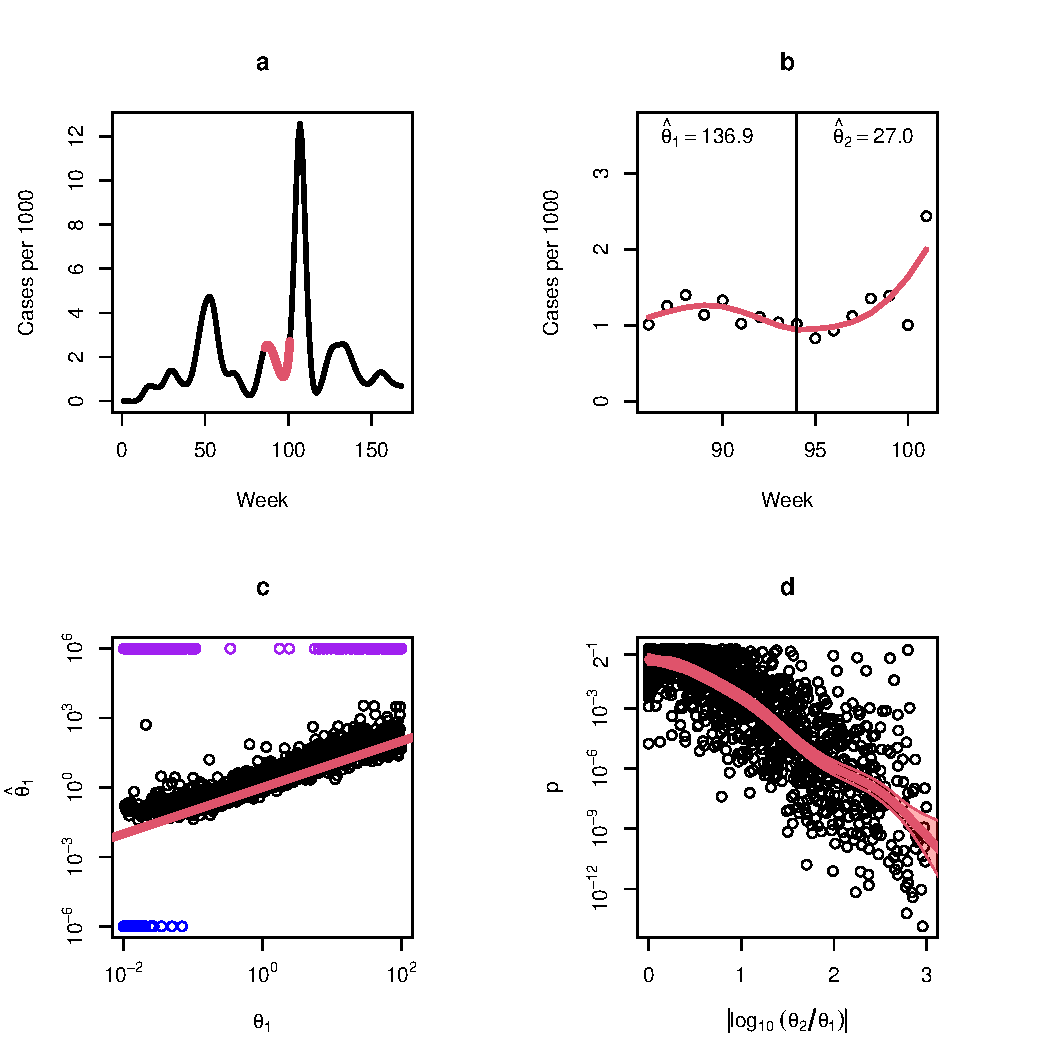
\includegraphics[width=1\textwidth]{fig1}
%\caption{
%Detecting changes in dispersion within incidence time series for populations of different sizes. (a, b) Simulated case counts with constant (a) and changing (b) dispersion parameters. (c, d) Dispersion parameters used to generate the data in (a) and (b), respectively. (e, f) LRT performance under varying absolute differences in \(\theta\) (horizontal axis), showing \( p \)-value distributions for population sizes of 50,000 (e) and 10,000,000 (f), representing the range in the empirical data. The null and alternative hypotheses (O and X) correspond to the parameters in (c) and (d). Red vertical lines indicate interquartile ranges.
%}\label{fig1}
%\end{figure}




\section*{Acknowledgments}
RA work on this project was supported by X and Y. BDD work on this project was supported by the National Science Foundation (NSF) grants (X, Y) and by the David and Lucile Packard Foundation.

\section*{References}
\bibliographystyle{vancouver} % Use plainnat or another appropriate style
\bibliography{references} % Create a references.bib file

% End Document
\end{document}
